\chapter{Tests}
Viele Gesichtserkennungsmodelle wurden mit Datensätzen trainiert, die ausschließlich Gesichter von realen Personen enthalten und für die Erkennung dieser optimiert. Modelle, die zuverlässig reale Gesichter detektieren, weisen bei der Anwendung auf Bilder historischer Gemälde häufig eine deutlich geringere Erkennungsgenauigkeit auf. Ziel der folgenden Tests ist es, die Eignung und Leistungsfähigkeit verschiedener Gesichtserkennungsmodelle für die Anwendung auf historischen Gemälden zu evaluieren. Begonnen wird mit den Stichprobentests, in welchen ungeeignete Modelle aussortiert werden sollen. Es folgen die Größentests, die dazu dienen, die Ergebnisse bei verschiedenen Auflösungen zu vergleichen. So soll sichergestellt werden, dass weitere Tests nur Bilder mit einer für die jeweiligen Modelle geeigneten Auflösung verwenden. Im Anschluss werden die \gls{confidence}-Grenzwerte der Modelle optimiert. Dafür werden die \gls{confidence}-Werte für erkannte Gesichter und False-Positives verglichen, um den bestmöglichen Grenzwert zu ermitteln. Im letzten Test werden alle Modelle direkt miteinander verglichen. Hierbei werden die False-Negatives, False-Positives sowie die Gesichter gezählt, die nur von einem Modell erkannt wurden.


\section{Stichprobentests}
Um Zeit und Aufwand zu sparen, wird in Stichprobentests die Eignung der verschiedenen Gesichtserkennungsmodelle überprüft. Ungeeignete Modelle werden am Ende dieser Stichprobentests ausgeschlossen. Hauptkriterium für die Eignung eines Modells ist die Fähigkeit, Gesichter auf historischen Gemälden zuverlässig zu erkennen. Als sekundäres Kriterium sollte die Anzahl an False Positives in einem vertretbaren Verhältnis stehen. Ein Modell, das zwar alle Gesichter erkennt, jedoch auch große Teile des restlichen Bildes fälschlicherweise als Gesichter markiert, erlaubt keine präzise Aussage darüber, ob sich ein Overlay auf einem Gesicht befindet. Weitgehend vernachlässigt wird der Aspekt der Rechenzeit. Im Kontext des \gls{cda} gilt es als wichtiger, Gesichter möglichst zuverlässig zu erkennen, als dies möglichst schnell zu tun. Hierfür wurden vier Werke ausgewählt: ein Einzelporträt, ein Zwei-Personen-Porträt, ein Drei-Personen-Porträt sowie ein Gruppenbild. Jedes Modell wird auf jedes der vier Werke angewendet, wodurch sich direkt ein erster Eindruck ergibt, wie gut sich die Modelle im Vergleich eignen. Durch die verschiedenen Bildtypen ist es zudem möglich, dass sich bereits Eignungen für bestimmte Bildkategorien abzeichnen. Schließlich dienen die Tests auch dazu, erste \gls{confidence}-Grenzwerte für die Modelle zu definieren.


\begin{itemize}
	\item \textbf{Haar-Cascade:} Haar-Cascade, genauer \monofett{haarcascade\_frontalface\_default.xml}, eignet sich in keiner Weise. Es scheitert sowohl daran, zuverlässig das Gesicht in einem Einzelporträt zu erkennen, als auch daran, mehrere Gesichter in einem Gruppenbild zu identifizieren. Zudem kommt es häufig zu False-Positives – teilweise werden mehr falsche als tatsächliche Gesichter markiert (siehe dazu Abbildung \ref{fig:haarStichprobe}). Haar-Cascade besitzt keinen direkt einstellbaren \gls{confidence}-Grenzwert, jedoch ein Äquivalent. Selbst bei Variation dieses Wertes liefert das Modell keine zuverlässigen Ergebnisse und scheidet somit bereits an dieser Stelle für weitere Versuche aus. Auffällig ist zudem, dass Haar-Cascade bei identischen Motiven mit höherer Auflösung noch schlechter abschneidet, da vermehrt False-Positives entstehen.
\begin{figure}[tbh]
 \centering
 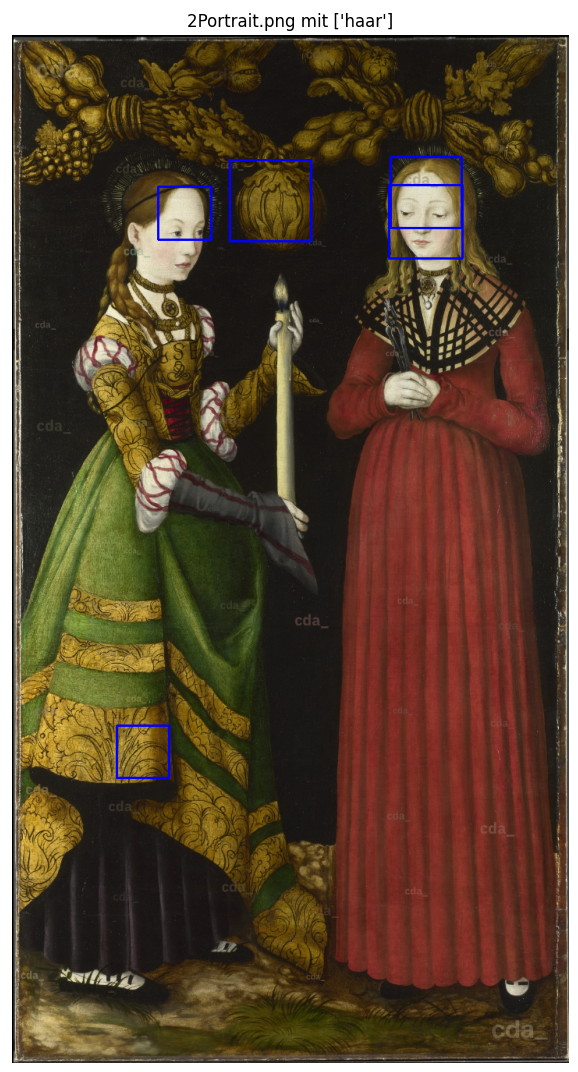
\includegraphics[width=0.4\textwidth]{Haar2Stichprobe}
 \caption{Stichprobenergebnis des Haar-Cascade-Modells bei einem Zwei-Personen-Porträt (Gemälde aus dem \gls{cda}, \cite{katharinenaltarGenovevaApollonia})}
 \label{fig:haarStichprobe}
\end{figure}
%	
	\item \textbf{Caffe:} Das \gls{caffe}-Modell besteht den Stichprobentest. In Einzel-, Zwei- und Drei-Personen-Porträts werden jeweils alle Hauptgesichter erkannt, ohne False-Positive (siehe dazu Abbildung \ref{fig:caffeStichprobe}). Allerdings zeigt das Modell Schwächen bei kleineren Gesichtern oder solchen, die nicht im Fokus des Porträts stehen. Im Gruppenbild wurde kein einziges Gesicht erkannt – auch keine False-Positives. Um Gesichter auf dem Gruppenbild zu erkennen, müsste der \gls{confidence}-Grenzwert so stark reduziert werden, dass die resultierenden False-Positives die Ergebnisse unbrauchbar machen würden. Bei höherer Auflösung ändern sich die Resultate kaum – nur im Gruppenbild treten mehr False-Positives auf, was die Problematik unterstreicht. Bei geringerer Auflösung erkennt Caffe weiterhin alle Gesichter korrekt und dies ohne False-Positives. Im Drei-Personen-Porträt wurde ein Nebengesicht nur halb erkannt. Überraschenderweise wurden im Gruppenbild mit geringer Auflösung tatsächlich Bereiche markiert. Dabei wurden einige Gesichter korrekt erkannt, jedoch waren die \gls{boundingbox}es zu groß, um sinnvoll nutzbar zu sein. Wiederholte Tests mit mittlerer Auflösung (600 × 1130 Pixel) zeigten, dass ein Nebengesicht im Drei-Personen-Porträt nicht erkannt wurde, obwohl dies bei höheren und niedrigeren Auflösungen gelang. Diese Inkonsistenz erschwert die Auswahl einer geeigneten Bildauflösung und könnte ein Grund sein, Caffe letztlich auszuschließen.
\begin{figure}[tbh]
 \centering
 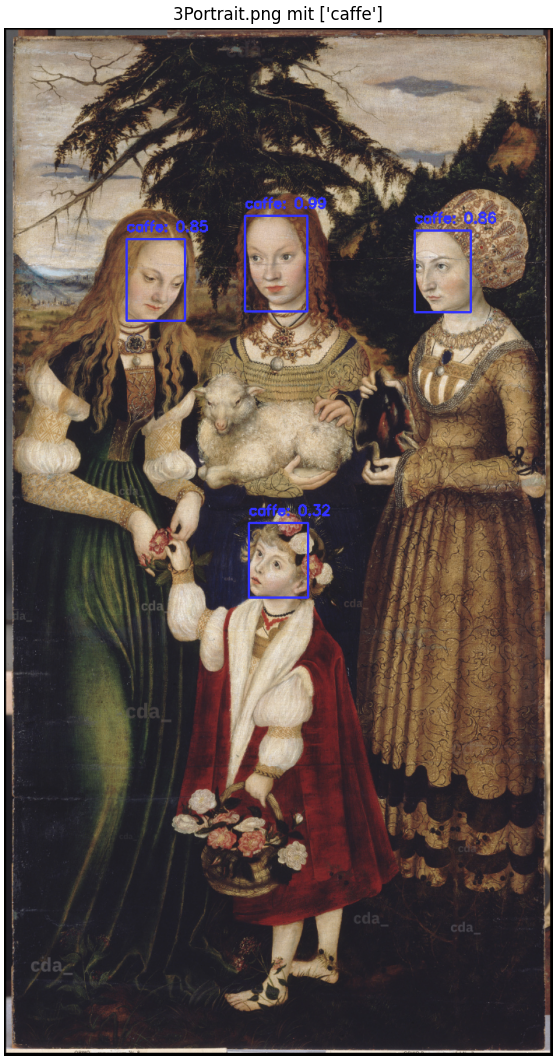
\includegraphics[width=0.4\textwidth]{Caffe3Stichprobe}
 \caption{Stichprobenergebnis des Caffe-Modells bei einem Drei-Personen-Porträt (Gemälde aus dem \gls{cda}, \cite{katharinenaltarDorotheaAgnesKunigunde})}
 \label{fig:caffeStichprobe}
\end{figure}
%	
	\item \textbf{MediaPipe:} MediaPipe erkennt das Gesicht im Einzelporträt zuverlässig und ohne False-Positives (siehe dazu Abbildung \ref{fig:mediaPipeStichprobe}). Dies ist jedoch der einzige bestandene Stichprobentest. In allen anderen Tests werden weder Gesichter noch False-Positives markiert. Das deutet darauf hin, dass MediaPipe nur große Gesichter erkennt. Da das Modell im gewünschten Kontext kaum brauchbar ist, wird es nicht weiter getestet. Auch bei höher aufgelösten Bildern bleiben die Ergebnisse identisch.
\begin{figure}[tbh]
 \centering
 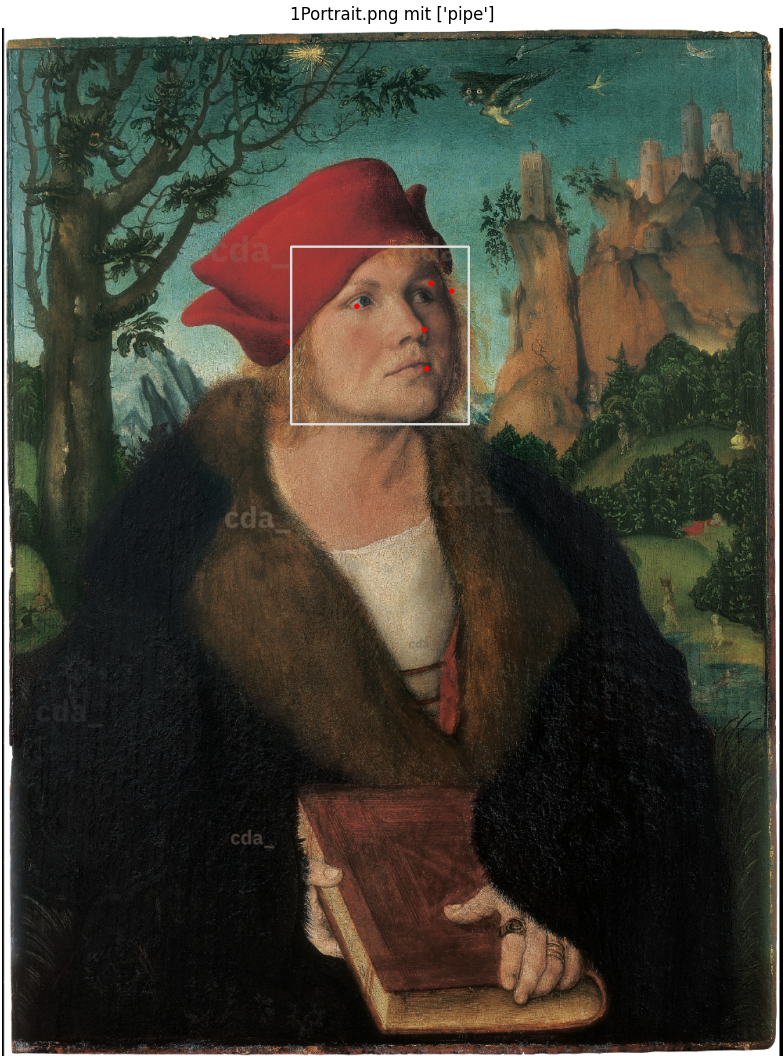
\includegraphics[width=0.4\textwidth]{MediaPipe1Stichprobe}
 \caption{Stichprobenergebnis des MediaPipe-Modells bei einem Einzelporträt (Gemälde aus dem \gls{cda}, \cite{bildnisCuspinian})}
 \label{fig:mediaPipeStichprobe}
\end{figure}
%	
	\item \textbf{Dlib HOG:} Das \gls{hog}-basierte Modell von dlib zeigt gute Leistungen bei der Erkennung kleiner Gesichter, hat jedoch Probleme mit größeren. Das Gesicht im Einzelporträt wird nur erkannt, wenn der \gls{confidence}-Grenzwert stark reduziert wird – was wiederum zu 0–3 False-Positives führt. Die Gesichter in Zwei- und Drei-Personen-Porträts sowie die meisten Gesichter im Gruppenbild werden hingegen gut erkannt (siehe dazu Abbildung \ref{fig:hogStichprobe}). Trotz offensichtlicher Schwächen sind die Ergebnisse solide genug für weiterführende Tests. Bei hochauflösenden Bildern erkennt das Modell auch das Einzelporträt, allerdings steigt die Zahl der False-Positives, ähnlich wie bei geringem \gls{confidence}-Grenzwert und niedriger Auflösung. Dies deutet darauf hin, dass der \gls{confidence}-Grenzwert abhängig von der Bildauflösung angepasst werden muss, was den Einsatzaufwand erhöht. Bei geringer Auflösung gibt es im Einzelporträt ein False-Positive, im Zwei- und Drei-Personen-Porträt jedoch keine. Im Gruppenbild verschlechtern sich die Ergebnisse deutlich: Statt 6 Gesichtern mit 3 False-Positives werden nur noch 1 Gesicht und 2 False-Positives erkannt. Das zeigt, dass Gruppenbilder und Porträts separat betrachtet werden sollten. Bei mittlerer Auflösung erkennt das Modell bei Einzel-, Zwei- und Drei-Personen-Porträts alle Gesichter mit 1–2 False-Positives pro Bild.
\begin{figure}[tbh]
 \centering
 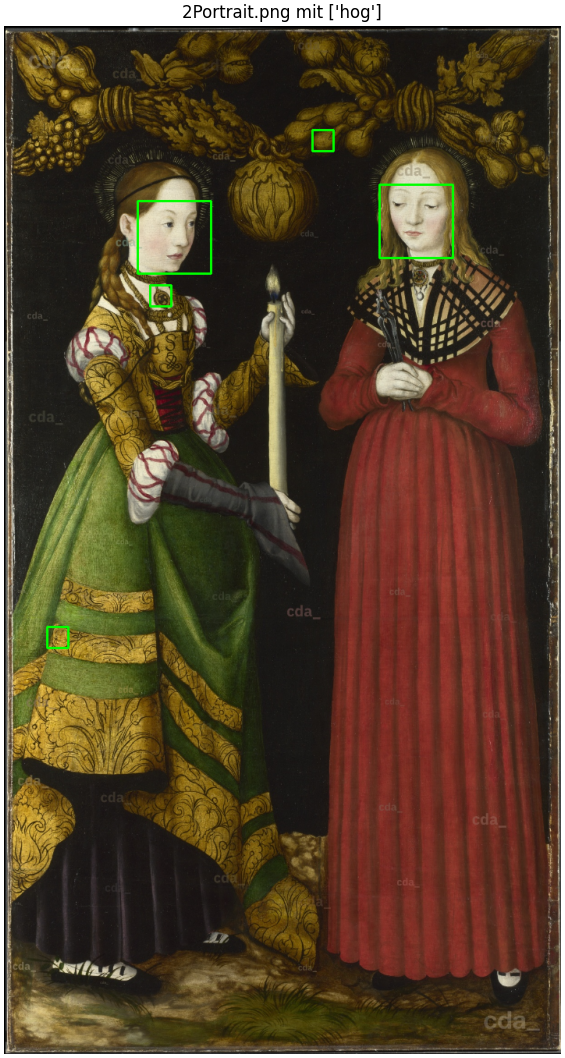
\includegraphics[width=0.4\textwidth]{Hog2Stichprobe}
 \caption{Stichprobenergebnis des Dlib-HOG-Modells bei einem Zwei-Personen-Porträt (Gemälde aus dem \gls{cda}, \cite{katharinenaltarGenovevaApollonia})}
 \label{fig:hogStichprobe}
\end{figure}
%	
	\item \textbf{Dlib HOG Landmark:} Anfangs wurde geplant, das Landmark-Modell ergänzend zur Überprüfung der Ergebnisse von Dlib \gls{hog} zu verwenden. Ziel war es, False-Positives auszusortieren und dadurch präzisere Ergebnisse zu erzielen. Diese Annahme bestätigt sich nicht. Zwar platziert das Modell die Landmarks korrekt, jedoch führt das Aussortieren basierend auf den Landmark-Daten häufig zur Entfernung korrekter Gesichter statt False-Positives (siehe dazu Abbildung \ref{fig:landmarkStichprobe}). Das Modell liefert somit keinen Vorteil gegenüber Dlib \gls{hog} und wird daher nicht weiter getestet. Auch hochauflösende Bilder verbessern die Ergebnisse nicht. Im Gegenteil, es entstehen häufig mehr False-Positives. Im Drei-Personen-Porträt wurde zwar ein zusätzliches Gesicht erkannt, die Gesamtleistung liegt dennoch unter der vom einfachem Dlib \gls{hog}.
\begin{figure}[tbh]
 \centering
 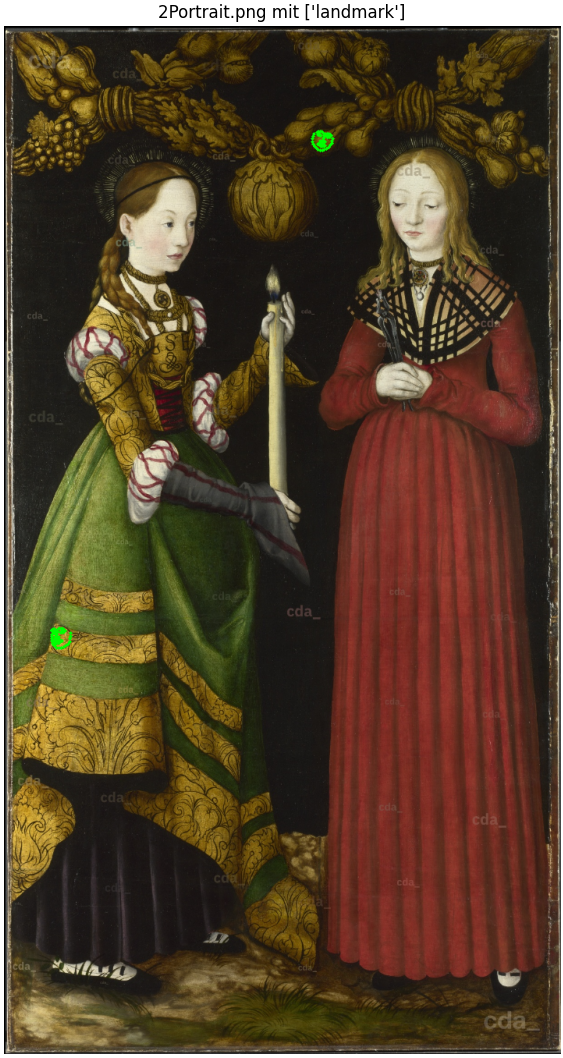
\includegraphics[width=0.4\textwidth]{Landmark2Stichprobe}
 \caption{Stichprobenergebnis des Dlib-HOG-Landmark-Modells bei einem Zwei-Personen-Porträt (Gemälde aus dem \gls{cda}, \cite{katharinenaltarGenovevaApollonia})}
 \label{fig:landmarkStichprobe}
\end{figure}
%	
	\item \textbf{Dlib CNN:} Dlib \gls{cnn}, konkret \monofett{mmod\_human\_face\_detector.dat}, ist das langsamste aller getesteten Modelle. Bereits bei Bildern mit einer Größe von 998 × 1314 Pixeln liegt die Bearbeitungszeit bei etwa 20 Sekunden, während alle anderen Modelle bei unter Drei Sekunden bleiben. Die Ergebnisse der Stichprobentests auf Porträts sind hingegen fehlerfrei (siehe dazu Abbildung \ref{fig:cnnStichprobe}). Im Gruppenbild wurde hingegen nichts erkannt. Aufgrund dieser hohen Zuverlässigkeit wird Dlib \gls{cnn} weiter getestet. Ob sich die lange Bearbeitungszeit durch eine entsprechend hohe Genauigkeit rechtfertigt, muss sich noch zeigen. Bei hochauflösenden Bildern (1200 × 1593 Pixel) bleiben die Ergebnisse gleich, allerdings verdoppelt sich die Bearbeitungszeit auf ca. 40 Sekunden. Bei geringer Auflösung (400 × 531 Pixel) arbeitet das Modell deutlich schneller, erkennt jedoch nur das Gesicht im Einzelporträt. Bei mittlerer Auflösung werden wieder alle Gesichter erkannt, mit Ausnahme des Nebengesichts im Drei-Personen-Porträt. Anders als viele andere Modelle lässt Dlib \gls{cnn} vermuten, mit höheren Auflösungen besser zu funktionieren, wobei es zu einer erheblich höheren Rechenzeit kommt.
\begin{figure}[tbh]
 \centering
 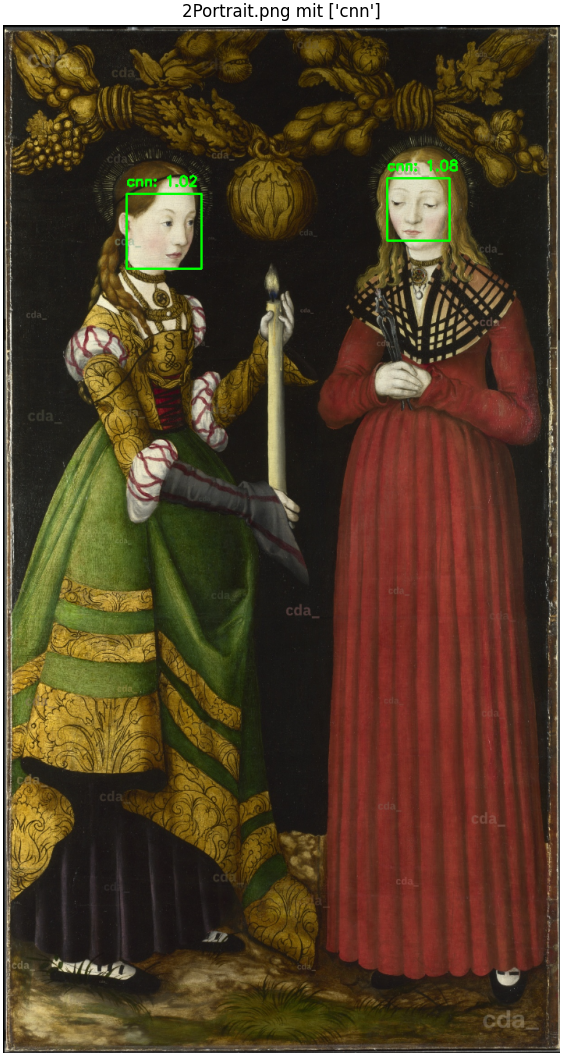
\includegraphics[width=0.4\textwidth]{Cnn2Stichprobe}
 \caption{Stichprobenergebnis des Dlib-CNN-Modells bei einem Zwei-Personen-Porträt (Gemälde aus dem \gls{cda}, \cite{katharinenaltarGenovevaApollonia})}
 \label{fig:cnnStichprobe}
\end{figure}
%	
	\item \textbf{MTCNN:} \gls{mtcnn} besteht die Stichprobentests für Einzel-, Zwei- und Drei-Personen-Porträts fehlerfrei (siehe dazu Abbildung \ref{fig:mtcnnStichprobe}). Im Gruppenbild werden einige Gesichter erkannt, allerdings nur solche mit \gls{confidence} > 0.5. Es gibt keine False-Positives. Somit wird MTCNN weiter getestet. Bei höherer Auflösung bleibt der durchschnittliche \gls{confidence}-Wert gleich, es treten jedoch in einzelnen Fällen 1–3 False-Positives auf. Im Gruppenbild werden mehr Gesichter erkannt (6 von 13), sowie keine neuen False-Positives. Einige dieser False-Positives haben hohe \gls{confidence}-Werte (0.85), was die Auswahl eines optimalen Schwellwerts erschwert. Bei geringer Auflösung erkennt MTCNN weiterhin zuverlässig alle Gesichter in Einzel-, Zwei- und Drei-Personen-Porträts mit einer \gls{confidence} von 1.0 und ohne False-Positives. Im Gruppenbild wird nichts markiert. Bei mittlerer Auflösung bleibt das Verhalten stabil – im Gruppenbild werden vier Gesichter mit ca. 0.85 \gls{confidence} erkannt.
\begin{figure}[tbh]
 \centering
 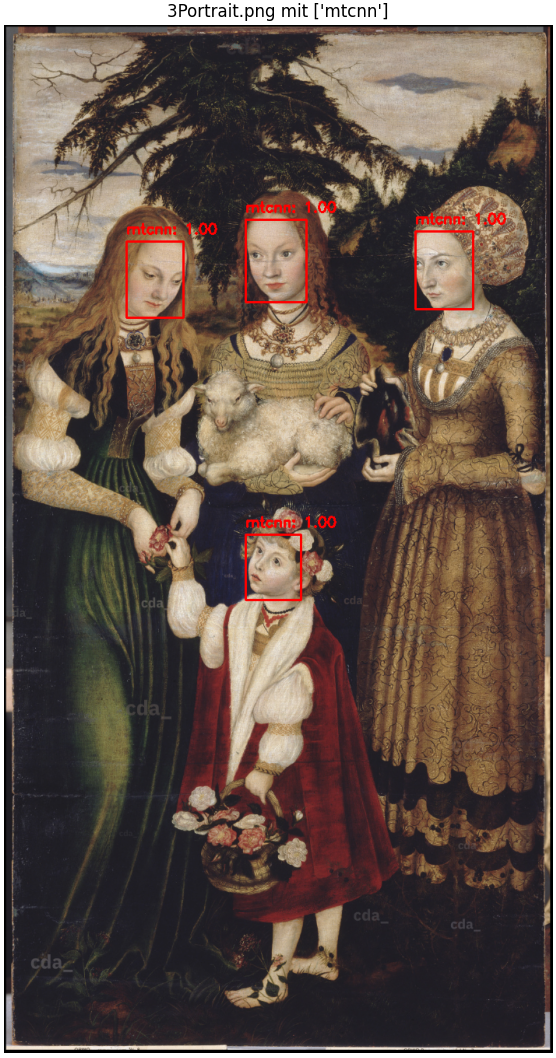
\includegraphics[width=0.4\textwidth]{Mtcnn3Stichprobe}
 \caption{Stichprobenergebnis des MTCNN-Modells bei einem Drei-Personen-Porträt (Gemälde aus dem \gls{cda}, \cite{katharinenaltarDorotheaAgnesKunigunde})}
 \label{fig:mtcnnStichprobe}
\end{figure}
%	
	\item \textbf{Yunet:} Das Yunet-Modell (\monofett{face\_detection\_yunet\_2023mar.onnx}) ist ohne Konfiguration sehr strikt. Es erkennt Gesichter mit hoher Präzision, ist aber auch sehr selektiv. Nach Einstellung des \gls{confidence}-Grenzwertes auf 0.8 werden alle Gesichter in Einzel-, Zwei- und Drei-Personen-Porträts erkannt (siehe dazu Abbildung \ref{fig:yunetStichprobe}), jedoch nur wenige im Gruppenbild. Ob 0.8 optimal ist, wird sich in weiteren Tests zeigen. Bei höherer Auflösung verbessert sich die \gls{confidence} der erkannten Gesichter leicht. Im Gruppenbild verändert sich die Erkennung – ein vorher erkanntes Gesicht fehlt, ein anderes wird zusätzlich erkannt. Es gibt weiterhin keine False-Positives. Bei geringer Auflösung erkennt Yunet alle Gesichter bis auf die im Gruppenbild, wo kein Gesicht markiert wird. Auch bei mittlerer Auflösung bleiben die Ergebnisse identisch zu jenen bei niedriger Auflösung.
\begin{figure}[tbh]
 \centering
 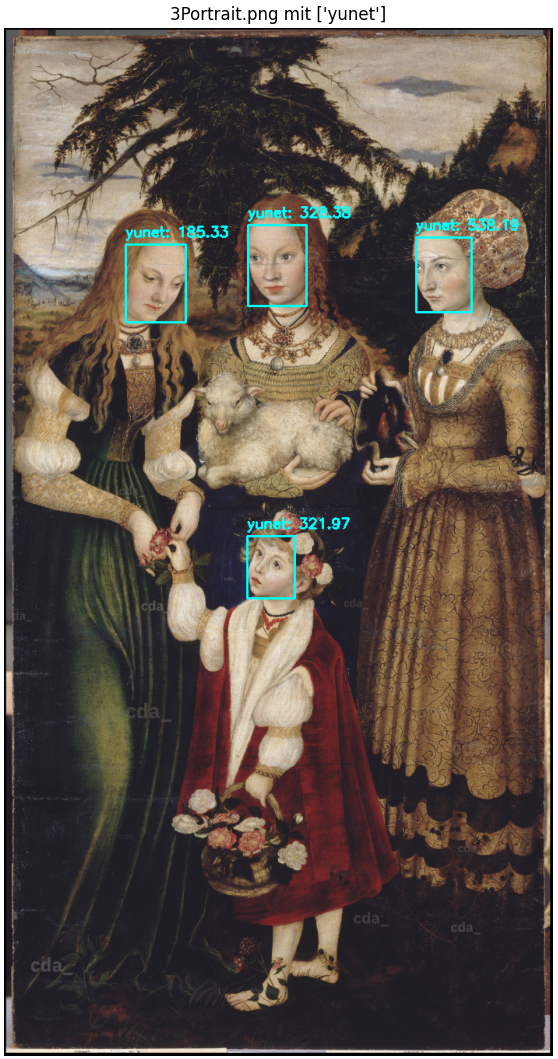
\includegraphics[width=0.4\textwidth]{Yunet3Stichprobe}
 \caption{Stichprobenergebnis des Yunet-Modells bei einem Drei-Personen-Porträt (Gemälde aus dem \gls{cda}, \cite{katharinenaltarDorotheaAgnesKunigunde})}
 \label{fig:yunetStichprobe}
\end{figure}
%	
	\item \textbf{RetinaFace (CPU):} Verwendet wird RetinaFace mit ResNet-50-\gls{backbone} und CPU-Nutzung, da GPU lediglich die Geschwindigkeit, nicht aber die Genauigkeit erhöht. RetinaFace erzielt in den Stichprobentests die besten Ergebnisse aller Modelle: Alle Gesichter in Einzel-, Zwei- und Drei-Personen-Porträts werden ohne False-Positives erkannt (siehe dazu Abbildung \ref{fig:retinaStichprobe}). Im Gruppenbild werden 10 von 13 Gesichtern identifiziert. Es treten zwei False-Positives auf, bei denen Pferdegesichter markiert wurden. Bei höherer Auflösung bleiben die Ergebnisse stabil, die \gls{confidence}-Werte ändern sich nur minimal. Im Gruppenbild wurde ein schwach erkanntes Gesicht nicht erneut erkannt. Bei geringer Auflösung erkennt RetinaFace weiterhin alle Gesichter in Einzel-, Zwei- und Drei-Personen-Porträts korrekt. Die Anzahl erkannter Gesichter im Gruppenbild sinkt auf 8 von 13, bleibt damit jedoch konkurrenzlos hoch. Auch bei mittlerer Auflösung bleiben die Erkennungsergebnisse stabil und präzise.
\begin{figure}[tbh]
 \centering
 \includegraphics[width=0.4\textwidth]{RetinaFace3Stichprobe}
 \caption{Stichprobenergebnis des RetinaFace-Modells bei einem Drei-Personen-Porträt (Gemälde aus dem \gls{cda}, \cite{katharinenaltarDorotheaAgnesKunigunde})}
 \label{fig:retinaStichprobe}
\end{figure}
\end{itemize}

\FloatBarrier
\section{Größentests}
Das \gls{cda} speichert Bilder von Werken in drei Größen: Small, Medium und Large. Da jedes Werk sein eigenes Format hat, haben nicht alle Bilder die exakt gleiche Auflösung. Small-Bilder haben 400~px Breite, Medium-Bilder haben 600~px Breite, Large-Bilder haben 1200~px Breite. Während der Stichprobentests wurde bereits ein wenig mit Bildern verschiedener Auflösungen experimentiert, die Ergebnisse waren jedoch nicht sehr übersichtlich oder eindeutig, sodass nochmal alle verbliebenen Modelle mit allen drei Größen getestet werden.

\begin{table}[tbh]
    \centering
    \resizebox{\textwidth}{!}{
    \begin{tabular}{|l|llllll|l|}
    \hline
        Portrait & Caffe & Dlib HOG & Dlib CNN & MTCNN & Yunet & RetinaFace & Gesammt \\ \hline
        1er S & A | 0 & 0 | 1 & A | 0 & A | 0 & A | 0 & A | 0 & -1 | 1 \\ 
        2er S & A | 0 & A | 0 & 0 | 0 & A | 0 & A | 0 & A | 0 & -2 | 0 \\ 
        3er S & 3 | 1 & A | 0 & 0 | 0 & A | 0 & A | 0 & A | 0 & -4 | 1 \\ \hline
        1er M & A | 0 & A | 1 & A | 0 & A | 0 & A | 0 & A | 0 & A | 1 \\ 
        2er M & A | 0 & A | 2 & A | 0 & A | 0 & A | 0 & A | 0 & A | 2 \\ 
        3er M & 3 | 0 & A | 1 & 3 | 0 & A | 0 & A | 0 & A | 0 & -2 | 1 \\ \hline
        1er L & A | 0 & A | 1 & A | 0 & A | 0 & A | 0 & A | 0 & A | 1 \\ 
        2er L & A | 0 & A | 7 & A | 0 & A | 0 & A | 0 & A | 0 & A | 7 \\ 
        3er L & A | 0 & A | 5 & A | 0 & A | 2 & A | 0 & A | 0 & A | 7 \\ \hline
    \end{tabular}
    }
    \caption{Ergebnisse des Größentests (Erkannte Gesichter [A = Alle erkannt] | False-Positives)}
 	\label{tab:groessenTabelle}
\end{table}

Als Ergebnis wird festgehalten, dass Large-Bilder sich am besten eignen. Diese haben den Nachteil, dass sie die meisten False-Positives generieren. Dennoch werden auf ihnen die meisten Gesichter erkannt (siehe dazu Tabelle \ref{tab:groessenTabelle}), was in diesem Anwendungskontext das relevantere Kriterium ist. Des Weiteren wird davon ausgegangen, dass einige dieser False-Positives darauf zurückzuführen sind, dass die \gls{confidence}-Grenzwerte noch nicht optimiert wurden. Dlib \gls{hog} wird verworfen, da es während der Tests im Vergleich deutlich mehr False-Positives gezeigt hat und es bereits genug Modelle mit akzeptablen Werten gibt, sodass das Modell als Kandidat nicht mehr relevant ist.

\section{Confidencetests}
Zur bestmöglichen Repräsentation der Modelle werden alle \gls{confidence}-Grenzwerte bzw. Score-Threshholds der Modelle angepasst. Zunächst wird kein Grenzwert gesetzt und die Ausgaben beobachtet. Dabei wird explizit auf die Werte des kleinsten \gls{confidence}-Wertes für ein erkanntes Gesicht und des höchsten \gls{confidence}-Wertes für ein False-Positiv geachtet. Sollten sich diese überschneiden, so wird mithilfe des Kontextes der anderen Ergebnisse bestimmt, welcher \gls{confidence}-Grenzwert sich für das jeweilige Modell am besten zur Gesichtserkennung auf historischen Gemälden eignet. Hier sei noch einmal angemerkt, dass jedes Modell seine eigene Implementierung für \gls{confidence}-Werte hat. Ein höherer Wert bedeutet jedoch nicht zwangsläufig, dass ein Modell besser ist – er gibt lediglich an, wie sicher sich das Modell ist, ein Gesicht erkannt zu haben.

\begin{table}[tbh]
    \centering
    \resizebox{\textwidth}{!}{
    \begin{tabular}{|l|lllll|}
    \hline
        Portrait & Caffe & Dlib CNN & MTCNN & Yunet & RetinaFace \\ \hline
        1er  & 0.11 | 0.21 & 1.03 | 0 & 0.99 | 0 & 389.12 | 0 & 0.74 | 0 \\ 
        2er  & 0.14 (0.13) | 0.40 & 0.70 | 0 & 0.82 | 0 & 233.79 | 0 & 0.71 | 0 \\ 
        3er & 0.10 | 0.28 & 0.97 | 0 & 0.91 (0.83) | 0.95 & 154.46 | 0 & 0.68 (0.52) | 0 \\ \hline
        Maximal & 0.10 | 0.4 & 0.70 | 0  & 0.82 | 0.95 & 154.46 | 0 & 0.68 (0.52) | 0 \\ \hline
    \end{tabular}
    }
    \caption{Ergebnisse der Confidencetests (Minimal Gesichtserkennung [inkl. Nebengesichter] | Maximal False-Positiv)}
 	\label{tab:confidenceTabelle}
\end{table}

\begin{itemize}
	\item \textbf{Caffe:} Die Ergebnisse von \gls{caffe} waren bei einem \gls{confidence}-Grenzwert von -1 viel zu unkenntlich, also wurde der Test wiederholt. Im zweiten Anlauf wurden alle Markierungen mit einem \gls{confidence}-Wert >= 0{,}1 akzeptiert, da alle Ergebnisse unter diesem Wert aufgrund der riesigen Mengen an False-Positives unbrauchbar wären.
Der minimale \gls{confidence}-Wert für erkannte Gesichter beim Einzelporträt ist 0{,}11, während der maximale False-Positive-Wert 0{,}21 ist. Dieser Wert wurde bei einem der Testbilder gemessen (siehe dazu Abbildung \ref{fig:caffeConfidence}), alle anderen erreichten einen Wert von 1 oder ca. 0{,}8. Da nur ein Bruchteil des Cranach-Archivs aufgrund der limitierten Zeit getestet werden kann, wird der Wert nicht als Ausreißer, sondern als gleichwertig betrachtet, da es im restlichen Archiv vermutlich ähnliche Bilder gibt.
\begin{figure}[tbh]
\centering
 \includegraphics[width=0.35\textwidth]{PhotoLog07}
 \caption{Confidenceergebnis des Caffe-Modells bei dem ein erkanntes Gesicht einen geringeren Wert als ein False-Positives hat (Gemälde aus dem \gls{cda}, \cite{hochaltarNicolaiDoebeln})}
 \label{fig:caffeConfidence}
\end{figure} 
Ergebnisse des Tests mit Zwei-Personen-Porträts waren deutlich weniger konstant als die des letzten Tests. Der geringste Wert für ein erkanntes Gesicht war 0{,}14 bzw. 0{,}13 wenn Nebengesichter mitgezählt werden. Allerdings gab es mit 0{,}4 ein großes False-Positive, sowohl vom Wert als auch von der Fläche her.  
Der Test mit Drei-Personen-Porträts verlief sehr schlecht für \gls{caffe}. Der geringste erkannte Wert ist 0{,}1. Es ist aber auch sehr wahrscheinlich, dass der eigentliche Wert noch geringer ist, da in manchen Bildern nicht alle Gesichter erkannt wurden. Auch gab es eine sehr große Menge an False-Positives mit einem höchst Wert von 0{,}28.  
Mit minimaler Gesichtserkennung bei \gls{confidence} von 0{,}1 und maximalem False-Positive-\gls{confidence} von 0{,}4 ist das Bestimmen eines optimalen Grenzwertes sehr schwierig. Nach mehreren weiteren Tests wird entschieden, den Grenzwert auf 0{,}14 zu setzen. Leider werden damit einige Ergebnisse von erkannten Gesichtern verworfen, allerdings gibt es bis 0{,}13 noch große Mengen an False-Positives, was die Gesamtergebnisse brauchbarer macht.
%	
	\item \textbf{Dlib CNN:} Dlib \gls{cnn}s Tests mit Einzelporträts haben selbst bei einem Grenzwert von -1 keine False-Positives gezeigt. Der minimale Wert für erkannte Gesichter liegt bei 1{,}03.  
Im Test mit Zwei-Personen-Porträts gab es weiterhin keine False-Positives, allerdings wurden auch einige Neben- sowie Hauptgesichter nicht erkannt. 0{,}7 ist der kleinste gemessene Wert für ein Gesicht.  
Weiter werden im Test mit Drei-Personen-Porträts keine False-Positives erkannt, aber auch teilweise Gesichter nicht erkannt. Der geringst gemessene Wert für ein erkanntes Gesicht war in diesem Test 0{,}97, womit 0{,}7 der gesamt niedrigste Wert für Dlib \gls{cnn} ist. Da bisher keine False-Positives erkannt wurden und Dlib \gls{cnn} sehr streng scheint, ist der verwendete Grenzwert für Dlib \gls{cnn} 0{,}6.
%	
	\item \textbf{MTCNN:} \gls{mtcnn} hat keine False-Positives und einen minimalen \gls{confidence}-Wert von 0{,}99 bei der Gesichtserkennung. Generell sind alle Werte konstant zwischen 0{,}99 und 1.  
Im Test mit Zwei-Personen-Porträts wurden weiterhin keine False-Positives erkannt, allerdings ebenso einige Gesichter nicht. Der geringste gemessene Wert bei der Gesichtserkennung beträgt 0{,}82. Die Ergebnisse des Tests mit Drei-Personen-Porträts erschweren das Bestimmen eines endgültigen Grenzwertes für \gls{mtcnn}. Der höchste Wert für False-Positives beträgt 0{,}95, generell haben alle False-Positives von \gls{mtcnn} sehr hohe \gls{confidence}-Werte (siehe dazu Abbildung \ref{fig:mtcnnConfidence}). Die Entscheidung, wo der Grenzwert gesetzt werden soll, fällt sehr schwer. Die beiden Möglichkeiten sind 0{,}82 für den minimalen Wert eines erkannten Gesichts oder 0{,}91, um den größten Teil der False-Positives auszusortieren. Der Grund, warum 0{,}82 überhaupt in Erwägung gezogen wird, ist, dass die markierten False-Positives Bereiche kleine sind und ignoriert werden könnten. Der Grenzwert wird vorläufig auf 0{,}82 gesetzt. Abhängig von den Ergebnissen wird das Modell mit 0{,}91 Grenzwert getestet und entschieden, welcher Wert verwendet wird.
\begin{figure}[tbh]
\centering
 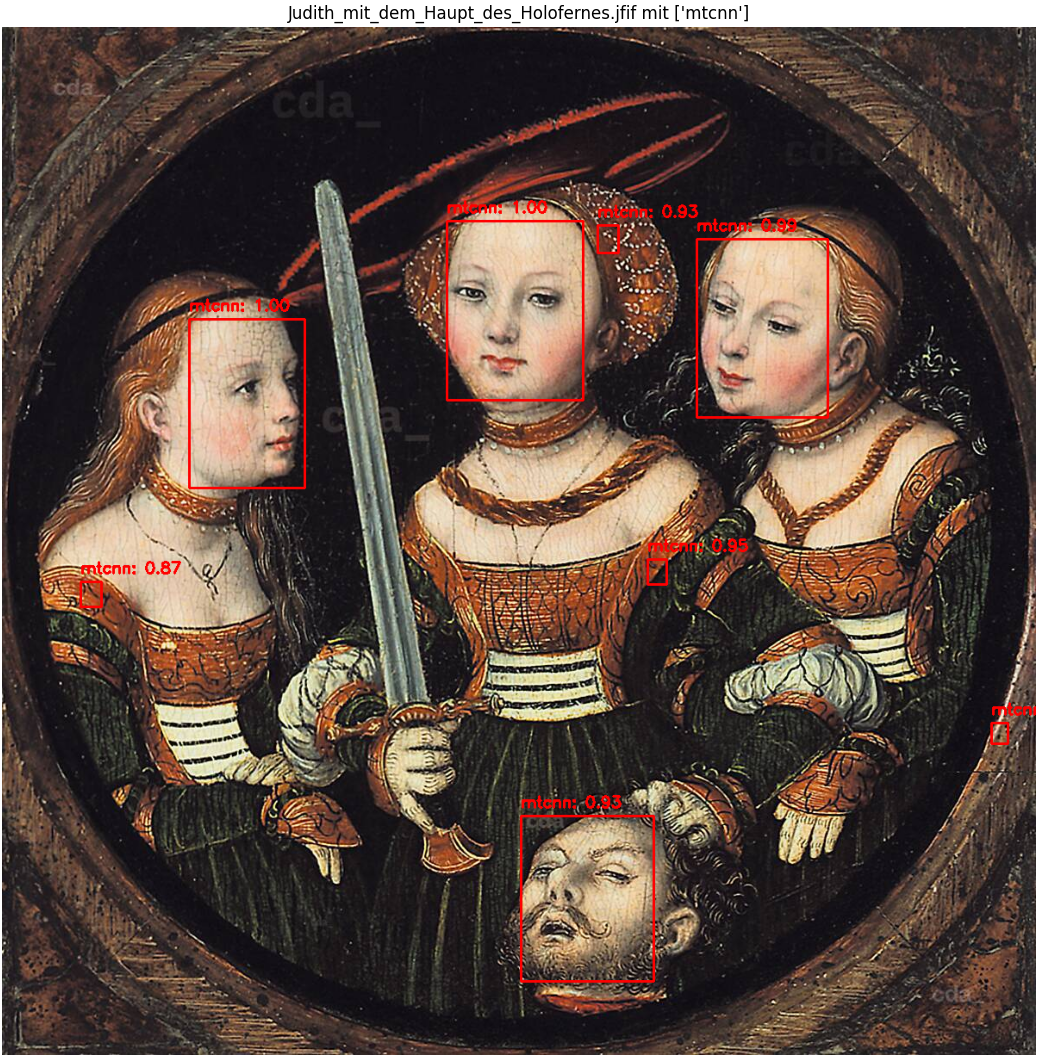
\includegraphics[width=0.6\textwidth]{Mtcnn3Confidence}
 \caption{Confidenceergebnis des MTCNN-Modells mit False-Positives (Gemälde aus dem \gls{cda}, \cite{cdaJudith})}
 \label{fig:mtcnnConfidence}
\end{figure} 
%	
	\item \textbf{Yunet:} Yunet hat bei seinem Einzelporträt-Test keine False-Positives gehabt und ein Gesicht übersehen, ansonsten betrug der minimale Wert für ein erkanntes Gesicht 389{,}12. Der Test mit Zwei-Personen-Porträts verlief mit einem ähnlichen Ergebnis und einem minimalen Wert von 233{,}79. Der letzte \gls{confidence}-Test von Yunet mit Drei-Personen-Porträts ergab weiterhin keine False-Positives und auch den gesamt minimalen Wert für erkannte Gesichter von 154{,}46. Da Yunet wie Dlib \gls{cnn} eher streng zu sein scheint, wird der Grenzwert für Yunet auf 125 gesetzt, um weitere mögliche erkannte Gesichter zuzulassen.
%	
	\item \textbf{RetinaFace (CPU):} RetinaFace hat als minimalen \gls{confidence}-Wert 0{,}74 für Gesichter im Test mit Einzelporträts, ohne Fehler. Die Ergebnisse für Zwei-Personen-Porträts zeigen einen minimalen Wert von 0{,}71 und keine False-Positives, es wurden aber auch manche Gesichter nicht erkannt. Das Ergebnis des Tests mit Drei-Personen-Porträts entspricht dem gesamt minimalen Wert von RetinaFace: 0{,}68 \gls{confidence} für Gesichter und 0{,}52 für Nebengesichter. Da in keinem Test False-Positives markiert wurden, wird der absolut geringst gemessene Wert 0{,}52 als Grenzwert verwendet.
\end{itemize}

\FloatBarrier
\section{Vergleich}
Keines der Modelle hat es geschafft, jedes Gesicht aus den bisherigen Tests fehlerfrei zu erkennen. Somit werden im letzten Test alle fünf verbliebenen Modelle gleichzeitig getestet. Dabei werden für jedes Modell die Anzahl von False-Negatives, False-Positives und die Anzahl von Gesichtern, die nur von diesem Modell erkannt wurden, gezählt (siehe dazu Tabelle \ref{tab:vergleichTabelle}). Ziel ist es, ein Modell oder eine kleine Auswahl von Modellen herauszuarbeiten, das genutzt werden kann, um so viele Gesichter wie möglich auf historischen Gemälden zu erkennen.

\begin{table}[tbh]
    \centering
    \begin{tabular}{|l|l|l|l|l|l|}
    \hline
        Portrait & Caffe & Dlib CNN & MTCNN & Yunet & RetinaFace \\ \hline
        1er  & -1 | 4 | 0 & 0 | 0 | 0 & 0 | 0 | 0 & -1 | 0 | 0 & 0 | 0 | 0 \\ 
        2er  & -1 | 2 | 0 & -2 | 0 | 0 & -2 | 0 | 0 & -2 | 0 | 0 & -2 | 0 | 0 \\ 
        3er & -11 | 3 | 0 & -10 | 0 | 1 & -4 | 6 | 7 & -4 | 0 | 0 & -2 | 0 | 2 \\ \hline
        Insgesammt & -13 | 9 | 0 & -12 | 0 | 1 & -6 | 6 | 7 & -7 | 0 | 0 & -4 | 0 | 2 \\ \hline
    \end{tabular}
    \caption{Ergebnisse der finalen Modelltests (False-Negatives [In negativen Zahlen dargestellt] | False-Positives | Gesichter die nur von diesem Modell erkannt wurden)}
 	\label{tab:vergleichTabelle}
\end{table}

Die Entscheidung, welches oder welche Modelle sich zur Weiterentwicklung eignen, ist keine einfache, da es kein fehlerfreies Modell gibt, das ohne Weiteres ausgewählt werden könnte. Auch kommt es in manchen Bildern vor, dass mehrere Gesichter jeweils von unterschiedlichen Modellen erkannt werden (siehe dazu Abbildung \ref{fig:modellVergleich}). Der ursprüngliche Ansatz war, je nach Bild den \gls{confidence}-Grenzwert und das Modell zu wählen. Hierbei bleibt jedoch weiterhin das Problem bestehen, dass kein einzelnes Modell alle Gesichter eines Bildes erkennt. Der neue Ansatz ist nun, je nach Bild mehrere Modelle zu- und abzuschalten, um auf diese Weise mehr Gesichter zu erkennen und False-Positives zu vermeiden. Unter Berücksichtigung des angestrebten Anwendungszwecks fällt die finale Wahl auf: RetinaFace (CPU), \gls{mtcnn} und \gls{cnn}. RetinaFace ist das Modell mit den wenigsten False-Negatives. Zusätzlich hat es auch keine False-Positives generiert, womit es als eine gute Basis dient. \gls{mtcnn} wurde gewählt, da es zusammen mit \gls{cnn} eines der Modelle ist, welches Gesichter markiert hat, die von keinem anderen Modell markiert wurden. Dabei wird der \gls{confidence}-Grenzwert von 0.82 beibehalten, da viele der besonders kleinen Gesichter nur von \gls{mtcnn} erkannt werden und unter den alternativen Wert von 0.91 fallen. Da \gls{mtcnn} abgeschaltet werden kann, falls die False-Positives stören, ist es dennoch eine gute Ergänzung zur Modellauswahl. \gls{cnn} wird aus dem gleichen Grund wie \gls{mtcnn} hinzugezogen. Es hat zwar keine False-Positives, die zu Problemen werden könnten, sollte jedoch nur bei Bedarf eingesetzt werden, da es die Rechenzeit deutlich erhöht. Weiter enthalten die Ergebnisse des Modells viele False-Negatives.
\begin{figure}[tbh]
\centering
 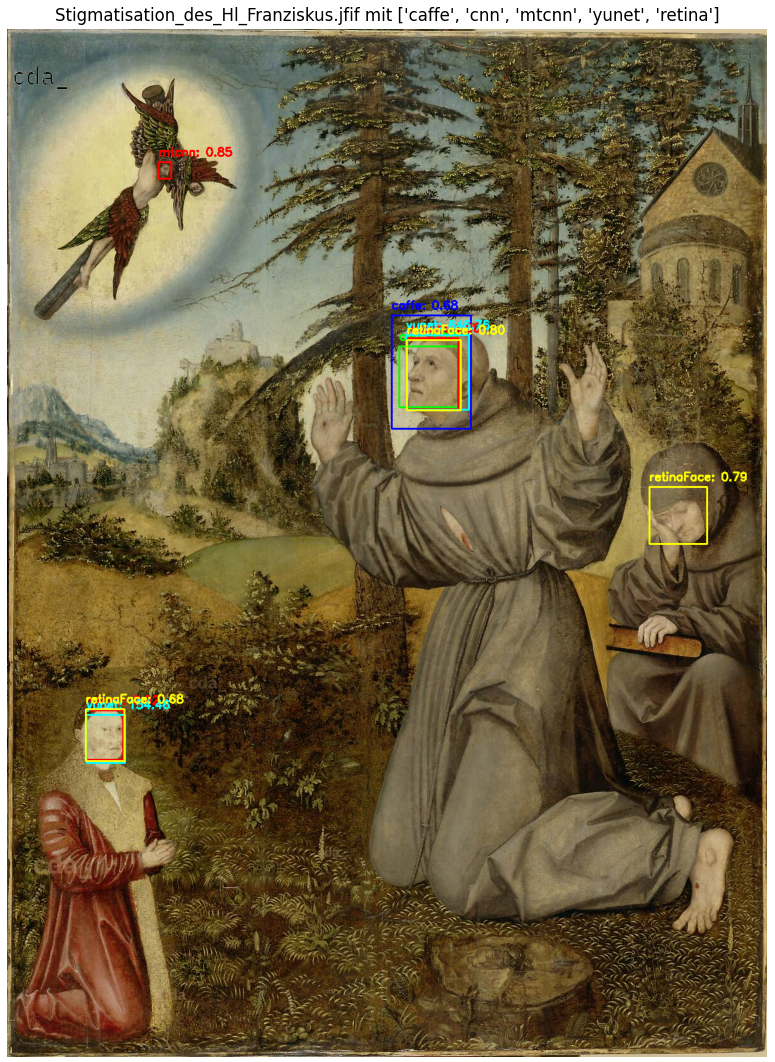
\includegraphics[width=0.6\textwidth]{PhotoLog08}
 \caption{MTCNN und RetinaFace haben jeweils Gesichter, die nur von ihnen markiert wurden (Gemälde aus dem \gls{cda}, \cite{stigmatisationFranziskus})}
 \label{fig:modellVergleich}
\end{figure} 